% Compile with pdflatex. The editable figure is included below.
\documentclass[11pt,letterpaper]{article}
\usepackage[T1]{fontenc}
\usepackage[utf8]{inputenc}
\usepackage{lmodern,microtype,tikz,hyperref,fancyhdr}
\usepackage[margin=0.88in,headheight=14pt,headsep=12pt]{geometry}
\usepackage[compact]{titlesec}
\definecolor{ink}{HTML}{1C4448}
\definecolor{steel}{HTML}{CBDCDA}
\definecolor{accent}{HTML}{883948}
\hypersetup{colorlinks=true,urlcolor=ink,linkcolor=ink}
\titleformat{\section}{\sffamily\Large\bfseries\color{ink}}{}{0pt}{}
\titleformat{\subsection}{\sffamily\normalsize\bfseries\color{ink}}{}{0pt}{}
\setlength{\parindent}{0pt}
\setlength{\parskip}{0.54em}
\setlength{\emergencystretch}{1.5em}
\pagestyle{fancy}\fancyhf{}\lhead{\small\sffamily NSF AMDO}\rhead{\small\sffamily Initial project description}\rfoot{\small\sffamily Collaborative working draft\quad\thepage}
\begin{document}


\section*{Defect Evolution in Hybrid Metal Manufacturing}

A repair shop can deposit stainless steel on a worn surface, scan the deposit using X-ray computed tomography (CT), and machine it back to the specified dimensions. From the scan, an inspector can estimate which buried pores the planned cut will expose. The estimate assumes that the cutter simply removes everything above a plane. If the tool pushes metal over a pore mouth, the finished opening may be smaller than predicted. Near an acceptance limit, that difference could change the grade of an entire face. We propose to establish when a virtual cut is a reliable basis for planning a repair and when material displacement makes a physical check worthwhile.

\subsection*{Objective and intellectual merit}

Our central hypothesis is that the geometry of a resolved pore and its orientation relative to tool travel help determine whether a finish cut leaves the mouth open or partly covers it. A competing explanation is that the CT scan mislocates the pore boundary or the tool reaches a slightly different depth. Both explanations can produce a smaller opening. Evidence for displacement would be a direction-dependent narrowing at the registered depth, together with deformation of the original rim. A pre-existing overhang or adhered cutting debris could also resemble a lip. The team’s 316L CNC micromilling experiments linked built-up material on the tool edge to deterioration of the surface finish [9]. We will record the cutting edge condition alongside the rim sections. Sectioning the rim gives us a way to distinguish these explanations.

\begin{center}

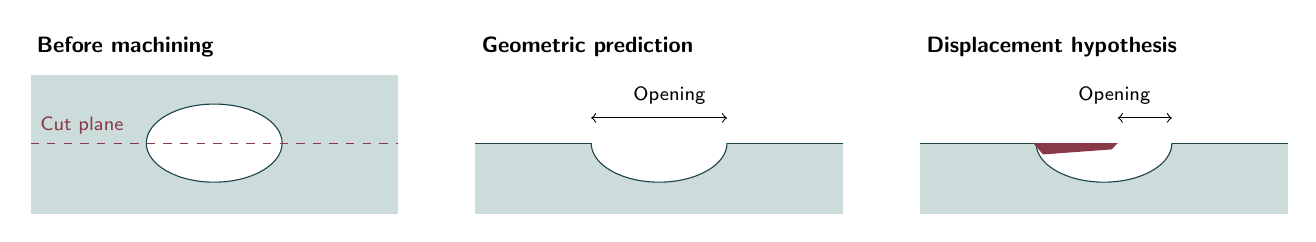
\begin{tikzpicture}[x=0.88cm,y=0.8cm,font=\sffamily\footnotesize]
\foreach \i/\label in {0/Before machining,1/Geometric prediction,2/Displacement hypothesis}{
  \begin{scope}[xshift=\i*5.65cm]
  \node[anchor=west,font=\sffamily\bfseries\footnotesize] at (-0.05,2.65){\label};
  \ifnum\i=0
    \fill[steel] (0,0) rectangle (5.3,2.2);
    \filldraw[fill=white,draw=ink] (2.65,1.12) ellipse (0.98 and 0.62);
    \draw[accent,dashed] (0,1.12)--(5.3,1.12);
    \node[accent,anchor=west,font=\sffamily\scriptsize] at (0,1.40){Cut plane};
  \else
    \fill[steel] (0,0) rectangle (5.3,1.12);
    \filldraw[fill=white,draw=ink] (1.67,1.12) arc[start angle=180,end angle=360,x radius=.98,y radius=.62];
    \draw[ink] (0,1.12)--(1.67,1.12) (3.63,1.12)--(5.3,1.12);
    \ifnum\i=2
      \fill[accent] (1.63,1.12)--(2.85,1.12)--(2.76,1.02)--(1.77,0.94)--cycle;
      \draw[<->] (2.85,1.52)--(3.63,1.52);
    \else
      \draw[<->] (1.67,1.52)--(3.63,1.52);
    \fi
    \node[font=\sffamily\scriptsize] at (2.8,1.88){Opening};
  \fi
  \end{scope}
}
\end{tikzpicture}

\end{center}

{\small\textbf{Figure 1.} Hypothetical cross-sections at the same cut depth. The geometric model exposes the pore. A displaced rim could narrow its visible mouth while the cavity persists below the surface.}

NIST identifies qualification after post-processing as a manufacturing measurement need [1]. In the team’s 316L stainless steel study, a deliberately porous block was machined at one finish depth [2]. That experiment leaves open what a different cut would expose. Prior machining studies document pore closure in porous titanium and adhered material on milled, deposited stainless steel [3, 4]. Finish turning has also reduced near-surface porosity in powder-bed 316L steel [7]. We will test a prediction, made before cutting, of which discrepancies will exceed measurement uncertainty and change a specified inspection grade on a new build.

Over three years we will measure how pore openings change, test a physical model where its predictions disagree with geometry alone, and evaluate the resulting inspection decision on independent builds. A useful outcome is a documented range in which ordinary geometric inspection already suffices.

\newpage

\section*{Aim 1 · Measure the physical effect of a finish cut}

% For Satish Bukkapatnam: Please specify a candidate drawing and its grading rule, the proposed pad/build schedule, a justifiable pair of cutting conditions and which facility can resolve and section the same pore. Clarify experimental scope relative to the funded FMRG work.
\textbf{Year 1.} Bukkapatnam’s group will establish a common coordinate system for the deposited pad, its pre-cut CT volume and its finished face. We will begin with a family of 316L pads deposited on separate build days. For the laboratory study we will record a continuous response, the visible width of a resolved opening in a specified section. Before sizing the application study, we will obtain the owner’s face rule. If it limits opening size, count or spacing, we will apply those clauses to the complete mapped face. Where an unresolved site could reverse the result, the prediction will be indeterminate and eligible for referral. A final surface grade applies to the face as delivered. A covered cavity can remain beneath it.

\subsection*{Establish the measurement limit}

Repeat scans and registrations will give a range of plausible pore boundaries at each site. We will measure the achieved plane independently and compute the range of opening widths that geometrical slicing alone would predict there. A low-deformation reference preparation on sacrificial specimens will test the registration and sectioning procedure. We will retain a separate “unresolved” class where plausible depths or boundaries span the grading limit. The relative contributions of CT resolution, depth and repeat inspection will determine which contrasts the available instruments can test.

\subsection*{Compare cuts and verify the mechanism}

We will block pads by build and randomly assign finish conditions within blocks before cutting. The first contrast will use two permissible tool-travel directions with a common target plane, tool specification and recorded edge condition. We will measure width along and across travel and record the signed shift of each rim edge in fixed specimen coordinates. Reversing travel could move a lip to the opposite edge without changing width. On a prespecified subset of asymmetric pores we will section the predicted leading and trailing edges. Multiple pore measurements from a pad describe one treated surface. New independently prepared pads supply replication. Zhang’s group will use variability among pads and builds in the pilot to size the subsequent experiment against a grading difference that matters to the owner.

Inspectors blinded to cutting condition and CT predictions will grade the intact faces. We will section selected rims and compare them with the low-deformation reference, looking for continuity and deformation of the original rim, adhered fragments or preparation damage. Ambiguous rims will retain an unresolved interpretation. A probability sample of apparent agreements will be sectioned alongside disagreements, since geometric and physical grades can agree for the wrong reason. We will record the sampling probabilities. These paired observations will define the range of pore sizes and depths for which competing mechanisms can be distinguished.

\newpage

\section*{Aim 2 · Predict when the geometric model fails}

% For Rui Tuo: Please define the geometric and displacement models, their identifiable calibration targets and the held-out contrast most likely to separate them. Identify which pre-cut quantities the shop can measure.
\textbf{Year 2.} Tuo’s group will build two predictions for the same candidate cut. The geometric model will intersect the reconstructed pore with plausible cut planes, using depth variation estimated on earlier trials. The alternative will allow movement of the rim to depend on local pore shape, travel direction and tool-edge condition. A constant offset fitted on discovery builds will supply a simple empirical competitor. The research question is whether accounting for contact between the tool and the rim changes a predicted grade under a new condition.

We will select a held-out contrast before seeing the corresponding faces. A particularly informative test is a pair of conditions where geometric exposure is similar but the displacement model predicts different openings. Bukkapatnam’s group will execute the contrast on independent pads. Zhang’s group will compare the predeclared predictions with continuous opening measurements and blinded face grades, carrying forward the unresolved class and the section-selection probabilities. Calibration and model checking will use different builds [5]. A model that improves average error but never changes the correct action near the grade limit offers little reason to change shop practice.

\section*{Aim 3 · Evaluate an inspection decision on new builds}

% For Xianyang Zhang: Please specify the build-level independent test, verification sampling and uncertainty for the whole-face grade. Indicate what can be inferred if some referred faces cannot be independently graded.
\textbf{Year 3.} With an application owner, we will specify a decision that can be taken before machining, such as referring a part for additional inspection before an expensive downstream operation. The owner will define the permissible action, grading rule and acceptable rate of missed rejects. The proposed rule can use only information available then. Achieved depth and destructive sections can explain a discrepancy after the fact and will remain unavailable to the routing rule.

On new builds, both rules will first issue referrals without changing the shop route. Inspectors will grade every finished face under the same protocol. This gives both rules the same reference and reveals false referrals and misses. If the owner permits a routing trial, we will randomly assign parts to model-guided referral, geometric referral or ordinary finish-and-inspect. An early check might avoid machining the rest of a surface later rejected. We will record the work actually avoided and the cost of the check, and audit referred and unreferred parts with known selection probabilities in each arm. Where a diverted part cannot receive a comparable reference grade, we will report bounds on missed rejects. We will estimate operational effects by assigned arm. Conditioning on achieved depth could bias this comparison if the route changes depth.

\newpage

\section*{Integration and broader impacts}

\subsection*{Feasibility and milestones}

Texas A\&M’s Institute for Manufacturing Systems lists an Optomec LENS MTS 500 hybrid system [6]. The team’s prior steel study establishes a build-and-cut route. It is listed under active Texas A\&M Future Manufacturing award 2328395 [8]. Before budgeting we will distinguish the proposed registered cuts, independent builds and verification costs from deliverables already funded. The first feasibility decision is whether a repair owner can identify one routine part, its applicable surface rule and an action worth taking earlier. The second is whether the proposed CT and sectioning facilities can resolve openings near that rule in this steel. These are proposed arrangements. Laboratory pads can support a mechanism study while the frequency and cost of consequential defects must be estimated on representative parts.

The first-year milestone is a registered, independently verified comparison whose uncertainty is narrow enough to interpret a change of grade. For the second, we will set a meaningful improvement with the owner before validation. We will use build-level uncertainty intervals to distinguish an improvement over both rivals, equivalence within the agreed margin, and insufficient precision. The third is a test of the frozen referral rule under the owner’s error tolerance. Even an ideal rule can avoid only the fraction of preventable losses multiplied by the downstream cost per loss. We will compare that ceiling with the incremental cost of CT, review and diversion under the shop’s existing inspection sequence. If the economics favor ordinary inspection, we will report the process conditions under which the simpler route is adequate.

\subsection*{Broader impacts}

We will develop an inspection exercise for manufacturing students and practicing inspectors using paired CT slices, finished-face images and verified sections. Participants will grade unseen faces and record whether they would request another observation before machining. Before and after instruction, participants will grade different, difficulty-matched faces. We will compare missed rejects and unnecessary referrals against independent grades and use the disagreements to revise the exercise. Laboratory-generated examples and their registration metadata can be released without requiring a partner to disclose a proprietary part drawing.

\subsection*{Selected sources}

\begin{enumerate}
\small\setlength{\itemsep}{0pt}
\item \href{https://www.nist.gov/programs-projects/additive-manufacturing-part-qualification}{NIST. Additive Manufacturing Part Qualification.}
\item \href{https://doi.org/10.1016/j.jmapro.2025.10.080}{Karthikeyan et al. Hybrid 316L deposition and machining study. Journal of Manufacturing Processes.}
\item \href{https://doi.org/10.1016/j.precisioneng.2022.04.010}{Ahmad et al. Micro-end-milling of porous titanium. Precision Engineering.}
\item \href{https://doi.org/10.1177/0954405420949360}{Tapoglou and Clulow. Milling of deposited 316L stainless steel.}
\item \href{https://arxiv.org/abs/2604.17144}{Li, Zhang and Tuo. Physical model validation against observations. Preprint, 2026.}
\item \href{https://texasmakes.tamu.edu/facilities/}{Texas A\&M Engineering Experiment Station. Institute for Manufacturing Systems facilities.}
\item \href{https://doi.org/10.3390/jmmp2020036}{Kaynak and Kitay. Porosity in 316L stainless steel after finish turning.}
\item \href{https://www.nsf.gov/awardsearch/showAward?AWD_ID=2328395}{NSF. Texas A\&M FMRG award 2328395 and its listed publications.}
\item \href{https://doi.org/10.1016/j.jmapro.2016.03.016}{Wang et al. Built-up-edge effects on surface deterioration in micromilling processes. Journal of Manufacturing Processes, 2016.}
\end{enumerate}

\end{document}
